\documentclass{beamer}

\usetheme{JuanLesPins}


\usepackage[utf8]{inputenc}

\usepackage{pgfplots}
\usepackage{pgfplotstable}
\usepackage{tikz}
\usepackage{xcolor}
\usetikzlibrary{automata, arrows.meta, shapes.geometric, positioning}

\usepackage{minted}
\usepackage{todonotes}
\usepackage[normalem]{ulem}
\usepackage[export]{adjustbox}



% \newtheorem{theorem}{Theorem}[chapter]
% \newtheorem{corollary}{Corollary}[theorem]
% \newtheorem{lemma}[theorem]{Lemma}
% \newtheorem{proposition}[theorem]{Proposition}
% \theoremstyle{definition}
% \newtheorem{example}[theorem]{Example}
% \newtheorem{definition}[theorem]{Definition}



\newcommand{\ZZ}{\mathbb{Z} \times \mathbb{Z}}
\newcommand{\nequiv}{\not\equiv}
\newcommand{\nequivp}{\nequiv_{\Psi,\T}}
\newcommand{\equivp}{\equiv_{\Psi,\T}}
% \renewcommand{\labelenumii}{\arabic{enumii}.}
\newcommand{\join}{\sqcup}
\newcommand{\meet}{\sqcap}
\newcommand{\widen}{\nabla}
\newcommand{\narrow}{\Delta}
\newcommand{\sem}[1]{\llbracket#1\rrbracket}
\newcommand{\Z}{\mathbb{Z}}
\renewcommand{\L}{\mathcal{L}}
\newcommand{\T}{\mathcal{T}}
\newcommand{\Set}{\mathcal{S}}
\newcommand{\oT}{{\overline{\mathcal{T}}}}
\newcommand{\F}{\mathcal{F}}
\newcommand{\A}{\mathcal{A}}
\newcommand{\X}{\mathcal{X}}
\newcommand{\V}{\mathcal{V}}
\newcommand{\malloc}{\textsf{malloc}}
\newcommand{\nf}{\textsf{nf}}
\newcommand{\restr}[2]{\left.\kern-\nulldelimiterspace#1\vphantom{|}\right|_{#2}}
\newcommand{\otau}{\overline{\tau}}
\newcommand{\angl}[1]{\langle#1\rangle}
% \newcommand{\widen}{\mathop{{\sqcup}\hspace*{-0.6em}\raisebox{.4ex}{\setlength{\unitlength}{1em}\line(1,0){.53}}}}
% \newcommand{\narrow}{\mathop{{\sqcap}\hspace*{-0.6em}\raisebox{.9ex}{\setlength{\unitlength}{1em}\line(1,0){.50}}}}
\newcommand{\ignore}[1]{}
\newcommand{\cpo}{\textsf{C-2PO}}
\newcommand{\goblint}{\textsc{Goblint}}
\newcommand{\find}[1]{\textsf{find}(#1)}
\newcommand{\union}[3]{\textsf{union}(#1, #2, #3)}
\newcommand{\closure}[4]{\textsf{closure}(#4, #1 = #2 + #3)}
\newcommand{\ext}[2]{\textsf{ext}\,{#1}\,{#2}}
\newcommand{\enter}{\textsf{enter}}
\newcommand{\combine}{\textsf{combine}}
\newcommand{\base}{\emph{base}}
\newcommand{\vareq}{\emph{var\_eq}}
\newcommand{\cpou}{$c$-$2po_1$}
\newcommand{\cpod}{$c$-$2po_2$}
\newcommand{\cpot}{$c$-$2po_3$}
\newcommand{\cpoq}{$c$-$2po_4$}


% Define TUM corporate design colors
% Taken from http://portal.mytum.de/corporatedesign/index_print/vorlagen/index_farben
\definecolor{TUMBlue}{HTML}{0065BD}
\definecolor{TUMSecondaryBlue}{HTML}{005293}
\definecolor{TUMSecondaryBlue2}{HTML}{003359}
\definecolor{TUMBlack}{HTML}{000000}
\definecolor{TUMWhite}{HTML}{FFFFFF}
\definecolor{TUMDarkGray}{HTML}{333333}
\definecolor{TUMGray}{HTML}{808080}
\definecolor{TUMLightGray}{HTML}{CCCCC6}
\definecolor{TUMAccentGray}{HTML}{DAD7CB}
\definecolor{TUMAccentOrange}{HTML}{E37222}
\definecolor{TUMAccentGreen}{HTML}{A2AD00}
\definecolor{TUMAccentLightBlue}{HTML}{98C6EA}
\definecolor{TUMAccentBlue}{HTML}{64A0C8}



\title[\cpo{}: A Weakly-Relational Pointer Analysis]{\cpo{}: A Weakly-Relational Pointer Analysis for the Goblint Abstract Interpreter}
\author{Rebecca Ghidini}
\date{\today}

\begin{document}
\maketitle

\section{Introduction}
\frame{\tableofcontents[currentsection]}

\begin{frame}{Motivation}
    \begin{itemize}
        \item Pointer analysis
        \item \emph{Weakly} relational: relations between pairs of pointer expressions, e.g.,
              \[
                  \&x = 4 + \&y
              \]
        \item \cpo{}: C-Analysis based on 2-Pointer Logic, introduced by Seidl et al.~\cite{2pointer}
    \end{itemize}
\end{frame}

\begin{frame}[containsverbatim]{Example}
    %(etwas was goblint noch nicht konnte auch nicht mit var eq
    %-> running example)
    \begin{minipage}{0.49\textwidth}

        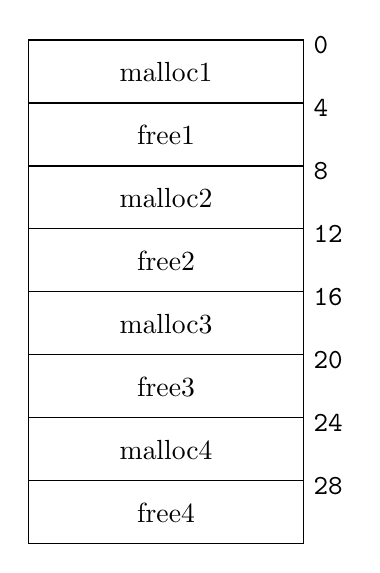
\begin{tikzpicture}

            % Settings
            \def\blockheight{0.8}
            \def\blockwidth{3.5}

            % Memory blocks and addresses
            \foreach \i/\label in {0/malloc1, 1/free1, 2/malloc2, 3/free2, 4/malloc3, 5/free3, 6/malloc4, 7/free4} {
                    % Draw memory block
                    \draw (0, -\i*\blockheight) rectangle (\blockwidth, -\i*\blockheight - \blockheight);
                    % Label the memory block
                    \node at (\blockwidth/2, -\i*\blockheight - \blockheight/2) {\label};
                    % Print address to the right
                    \node[above right=0.1cm and 0cm] at (\blockwidth, -\i*\blockheight - \blockheight/2) {\texttt{\the\numexpr 4*\i \relax}};
                }
        \end{tikzpicture}
    \end{minipage}
    \begin{minipage}{0.49\textwidth}

        \begin{minted}{C}
...
(*malloc)(p);
...
(*free)(p);
...
\end{minted}
        $\rightarrow$ $free = 4 + malloc$?
    \end{minipage}
\end{frame}

\begin{frame}{Disequalities}
    \[
        x \neq 4 + y
    \]
    \[
        bl(x) = bl(y)
    \]
    \begin{itemize}
        \item To know which terms are not modified by an assignment
        \item Block disequalities: terms are not in the same block/memory object
    \end{itemize}
\end{frame}

\section{Abstract Domain}
\frame{\tableofcontents[currentsection]}

\begin{frame}{Abstract Domain}
    \begin{itemize}
        \item Set of terms $\T$
              $\{A, *A, \&x, x, \&y, y, *(1+y)\}$
        \item Conjunction of equalities and disequalities:
              \begin{itemize}
                  \item Quantitative equalities
                        \[
                            (x = 1 + A) \land (\&x = \&y)
                        \]
                  \item Quantitative disequalities
                        \[
                            (x \neq 4 - y)
                        \]
                  \item Block disequalities
                        \[
                            (bl(y) \neq bl(A))
                        \]
              \end{itemize}
    \end{itemize}
\end{frame}

\begin{frame}{Quantitative Finite Automaton (QFA)}
    \[
        \T=\{ \&x, x, *x, A, *(1 + A), \&y\}
    \]
    \[
        (x = 1 + A) \land (\&x = \&y)
    \]
    \centering
    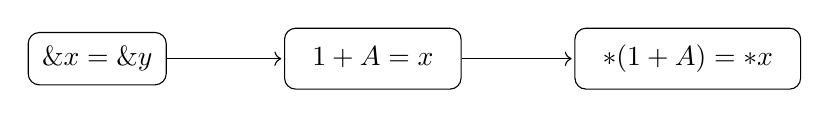
\begin{tikzpicture}[shorten >=1pt, node distance=5cm, on grid, auto, state/.style={rectangle, rounded corners, draw, inner sep=5pt, align=center}]

        \node[state] (y) {$\&x =\&y$};

        \node[state, right=3.5cm of y] (AB) {$\begin{array}{c}
                    1 + A = x
                \end{array}$};

        \node[state, right=4cm of AB] (ABs) {$\begin{array}{c}
                    *(1+A) = *x
                \end{array}$};

        \path[->]
        (y) edge[] (AB)
        (AB) edge[] (ABs);


    \end{tikzpicture}
\end{frame}

\begin{frame}{QFA: Insert Terms}
    \[
        \T=\{\&x, x, *x, A, *(1 + A), \&y, \textcolor{TUMAccentOrange}{y, *y}\}
    \]
    \[
        (x = 1 + A) \land (\&x = \&y)
    \]
    \centering
    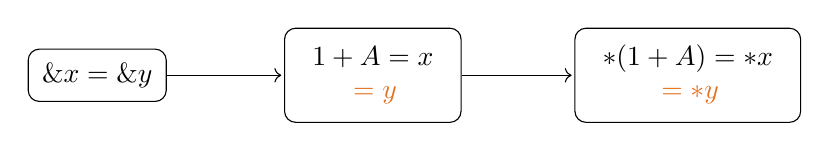
\begin{tikzpicture}[shorten >=1pt, node distance=5cm, on grid, auto, state/.style={rectangle, rounded corners, draw, inner sep=5pt, align=center}]

        \node[state] (y) {$\&x =\&y$};

        \node[state, right=3.5cm of y] (AB) {$\begin{array}{c}
                    1 + A = x \\
                    \textcolor{TUMAccentOrange}{\,= y}
                \end{array}$};

        \node[state, right=4cm of AB] (ABs) {$\begin{array}{c}
                    *(1+A) = *x \\
                    \textcolor{TUMAccentOrange}{\,= *y}
                \end{array}$};

        \path[->]
        (y) edge[] (AB)
        (AB) edge[] (ABs);


    \end{tikzpicture}


\end{frame}

\begin{frame}{QFA: Remove Terms}
    \[
        \T=\{\text{\textcolor{TUMAccentOrange}{\sout{$\&x, x, *x,$}}}A, *(1 + A), \&y\}
    \]
    \[
        (x = 1 + A) \land (\&x = \&y)
    \]
    \centering
    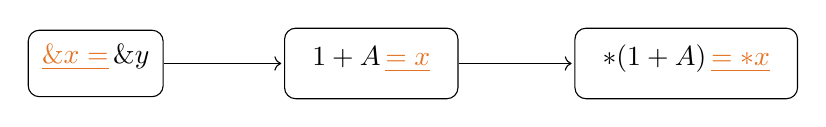
\begin{tikzpicture}[shorten >=1pt, node distance=5cm, on grid, auto, state/.style={rectangle, rounded corners, draw, inner sep=5pt, align=center}]

        \node[state] (y) {$\text{\textcolor{TUMAccentOrange}{\sout{\&x=}}} \,\&y$};

        \node[state, right=3.5cm of y] (AB) {$\begin{array}{c}
                    1 + A \, \text{\textcolor{TUMAccentOrange}{\sout{= x}}}
                \end{array}$};

        \node[state, right=4cm of AB] (ABs) {$\begin{array}{c}
                    *(1+A) \, \text{\textcolor{TUMAccentOrange}{\sout{= *x}}}
                \end{array}$};

        \path[->]
        (y) edge[] (AB)
        (AB) edge[] (ABs);


    \end{tikzpicture}

\end{frame}

\begin{frame}[containsverbatim]{Block Disequalities}
    \begin{itemize}
        \item Two terms do not belong to the same C block
        \item For all variables $x$ and $y$:
              \[
                  bl(\&x) \neq bl(\&y)
              \]
        \item
              \begin{minted}{C}
int *x = malloc();
int *y = malloc();
\end{minted}

              \[
                  bl(x) \neq bl(y)
              \]

    \end{itemize}
\end{frame}

\begin{frame}[containsverbatim]{Quantitative Disequalities}
    \begin{itemize}
        \item Deriving from block disequalities: If $bl(t_1) \neq bl(t_2)$
              \[
                  t_1\neq z+ t_2 \quad\quad \text{for each $z \in \Z$}
              \]
        \item Deriving from equalities: If $t_1 = z + t_2$,
              \[
                  t_1\neq z' + t_2 \quad\quad \text{for each $z' \neq z$}
              \]

        \item Deriving from guards:
              \begin{minted}{C}
if(*x != 4 + y){...}
\end{minted}
        \item Deriving from other disequalities: If $*(z_1 + t_1) \neq *(z_2 + t_2)$,
              \[ t_1 \neq (z_2 - z_1) + t_2
              \]
    \end{itemize}
\end{frame}

\section{Meet}
\begin{frame}{Meet}
    \begin{itemize}

        \item Equivalent to conjunction $\land$
        \item Update partition and QFA
        \item Add block/quantitative disequalities
        \item Closure of disequalities

    \end{itemize}
\end{frame}

\section{Join}
\begin{frame}{Join}
    \[
        \T = \{
        \&x,x,*x, {*}{*}x
        \}
    \]
    \begin{minipage}{0.4\textwidth}
        \centering
        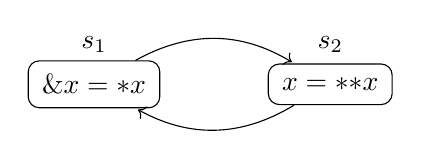
\begin{tikzpicture}[shorten >=1pt, node distance=3cm, on grid, auto, state/.style={rectangle, rounded corners, draw, inner sep=5pt, align=center}]

            \node[state, initial text={}] (Q1) {$\&x= *x$};
            \node[state, right=of Q1] (Q2) {$x= {*}{*}x$};
            \node[above=0.5cm of Q1] (s1) {$s_1$};
            \node[above=0.5cm of Q2] (s2) {$s_2$};


            \path[->]
            (Q1) edge[bend left, above] (Q2)
            (Q2) edge[bend left, below] (Q1);

        \end{tikzpicture}

        \vspace*{1cm}

        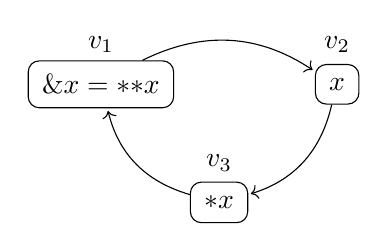
\begin{tikzpicture}[shorten >=1pt, node distance=3cm, on grid, auto, state/.style={rectangle, rounded corners, draw, inner sep=5pt, align=center}]

            \node[state, initial text={}] (Q1) {$\&x= {*}{*}x$};
            \node[state, right=of Q1] (Q2) {$x$};
            \node[state, below right=1.5cm and 1.5cm of Q1] (Q3) {$*x$};
            \node[above=0.5cm of Q1] (s1) {$v_1$};
            \node[above=0.5cm of Q2] (s2) {$v_2$};
            \node[above=0.5cm of Q3] (s3) {$v_3$};

            \path[->]
            (Q1) edge[bend left] (Q2)
            (Q2) edge[bend left] (Q3)
            (Q3) edge[bend left] (Q1);

        \end{tikzpicture}
    \end{minipage}
    \begin{tikzpicture}[overlay]
        \draw[->, thick] (0, 0) -- (1, 0);
    \end{tikzpicture}
    \hfill%
    \begin{minipage}{0.49\textwidth}

        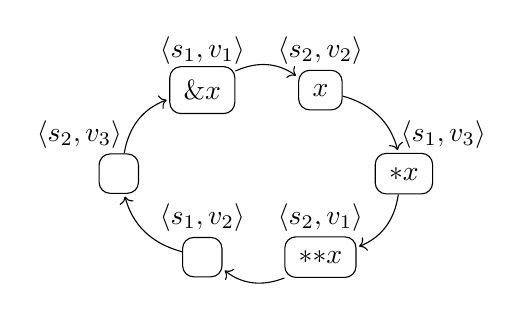
\begin{tikzpicture}[shorten >=1pt, node distance=1.5cm, on grid, auto, state/.style={rectangle, rounded corners, draw, inner sep=5pt, align=center, minimum size=0.5cm}]

            \node[state, initial text=] (Q1) {$\&x$};
            \node[state, right= 1.5cm of Q1] (Q2) {$x$};
            \node[state, below right=of Q2] (Q3) {$*x$};
            \node[state, below left=of Q3] (Q4) {${*}{*}x$};
            \node[state, left=of Q4] (Q5) {};
            \node[state, above left=of Q5] (Q6) {};
            \node[above=0.5cm of Q1] (s1) {$\angl{s_1,v_1}$};
            \node[above=0.5cm of Q2] (s2) {$\angl{s_2,v_2}$};
            \node[above right=0.5cm and 0.5cm of Q3] (s3) {$\angl{s_1,v_3}$};
            \node[above=0.5cm of Q4] (s4) {$\angl{s_2,v_1}$};
            \node[above=0.5cm of Q5] (s5) {$\angl{s_1,v_2}$};
            \node[above left=0.5cm and 0.5cm of Q6] (s6) {$\angl{s_2,v_3}$};



            \path[->]
            (Q1) edge[bend left] (Q2)
            (Q2) edge[bend left] (Q3)
            (Q3) edge[bend left] (Q4)
            (Q4) edge[bend left] (Q5)
            (Q5) edge[bend left] (Q6)
            (Q6) edge[bend left] (Q1)
            ;

        \end{tikzpicture}
    \end{minipage}
\end{frame}


\begin{frame}{Join}
    \begin{itemize}
        \item Add a term for each empty state in the automaton
    \end{itemize}
    \[
        \T = \{
        \&x,x,*x, {*}{*}x,\textcolor{TUMAccentOrange}{{*}{*}{*}x,{*}{*}{*}{*}x}
        \}
    \]

    \centering
    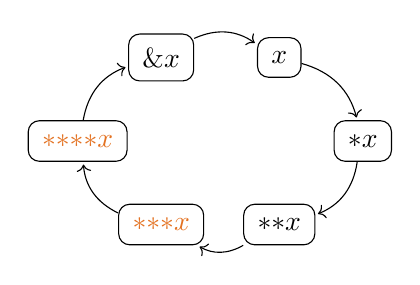
\begin{tikzpicture}[shorten >=1pt, node distance=1.5cm, on grid, auto, state/.style={rectangle, rounded corners, draw, inner sep=5pt, align=center, minimum size=0.5cm}]

        \node[state, initial text=] (Q1) {$\&x$};
        \node[state, right= 1.5cm of Q1] (Q2) {$x$};
        \node[state, below right=of Q2] (Q3) {$*x$};
        \node[state, below left=of Q3] (Q4) {${*}{*}x$};
        \node[state, left=of Q4] (Q5) {$\textcolor{TUMAccentOrange}{{*}{*}{*}x}$};
        \node[state, above left=of Q5] (Q6) {$\textcolor{TUMAccentOrange}{{*}{*}{*}{*}x}$};
        \path[->]
        (Q1) edge[bend left] (Q2)
        (Q2) edge[bend left] (Q3)
        (Q3) edge[bend left] (Q4)
        (Q4) edge[bend left] (Q5)
        (Q5) edge[bend left] (Q6)
        (Q6) edge[bend left] (Q1)
        ;

    \end{tikzpicture}
\end{frame}

\section{Widening and Narrowing}
\begin{frame}{Widening}
    \begin{itemize}
        \item Infinite strictly ascending chain:
    \end{itemize}
    \[
        \Psi_n \equiv (*^{2^n} \&x = \&x)\hspace{6pt} (n\geq 0).
    \]
    \begin{itemize}
        \item Limit the terms of the result to the set of terms of the first element
    \end{itemize}
    \[\Psi_1 \widen \Psi_2 = \restr{(\Psi_1 \join \Psi_2)}{\T_1}.\]
\end{frame}

\begin{frame}{Narrowing}
    \begin{itemize}
        \item Infinite strictly descending chains:
    \end{itemize}
    \[
        \Phi_n \equiv\bigwedge_{i=1}^n (\&y = *(i+\&x))\qquad(n\geq 0)
    \]
    \[
        \Psi_n \equiv (y\neq n+\&x)\qquad(n\geq 0)
    \]
    \begin{itemize}
        \item Limit the terms of the result and the possible offsets
              appearing in disequalities -> to what?
    \end{itemize}

\end{frame}

\section{Assignment}

\begin{frame}{Assignment}
    \[
        t_1\,{:=}\,?
    \]
    \begin{itemize}
        \item Forget all terms that may be modfied $\rightarrow$ terms that have the same address
        \item If $t_1 = A$ or $t_1 = \&x$: remove terms that have $t_1$ as subterm
        \item If $t_1 = *(z + t)$: keep only terms $*(z' + v)$ where $t \neq (z' - z) + v$
              \begin{itemize}
                  \item $t = z_1 + v$ and $z_1 \neq (z' - z)$ and they do not overlap
                  \item $t \neq (z' - z) + v$ or $bl(t) \neq bl(v)$
                  \item use non-relational analysis: possible values of $t$ and $(z' - z) + v$ do not intersect
              \end{itemize}
    \end{itemize}
\end{frame}

\begin{frame}{Assignment}
    \[
        t_1\,{:=}\,z + t
    \]
    \begin{itemize}
        \item Fresh auxiliary $A$
        \item Add equality $A = z + t$
        \item Remove terms modified by an assignment to $t_1$
        \item Add equality $t_1 = A$
        \item Remove $A$
    \end{itemize}
\end{frame}

\begin{frame}{Assignment}
    \[
        t_1\,{:=}\,\malloc
    \]
    \begin{itemize}
        \item For each $t \in \T$, add:
              \[
                  bl(t) \neq bl(t_1)
              \]
    \end{itemize}
\end{frame}

\section{Evaluation}
\frame{\tableofcontents[currentsection]}

\begin{frame}{Precision}
    \begin{itemize}
        \item 29 litmus tests, manually annotated invariants
        \item GNU Core Utilities, automatically annotated invariants by \cpo\
        \item Compared three different \goblint\ analyses:
              \begin{itemize}
                  \item \base{}: basic goblint analysis, including a non-relational pointer analysis
                  \item \vareq{}: tracks must-equalities between general expressions
                  \item \cpo\ implementation in \goblint\
              \end{itemize}
    \end{itemize}
\end{frame}


\begin{frame}{Litmus Tests}
    \begin{tikzpicture}
        \begin{axis}[
                ybar,
                symbolic x coords={\base, \vareq, \cpo},
                xtick=data,
                ymin=0, ymax=109,
                bar width=1cm,
                ylabel={Number of Proven Assertions},
                xlabel={Analyses},
                nodes near coords,
                nodes near coords align={vertical},
            ]
            \addplot coordinates {(\base, 17) (\vareq, 23) (\cpo, 109)};
        \end{axis}
    \end{tikzpicture}

\end{frame}

\begin{frame}{Coreutils Tests}
    \begin{tikzpicture}
        \begin{axis}[
                ybar,
                symbolic x coords={\base, \vareq, \cpo},
                xtick=data,
                ymin=0, ymax=19488,
                bar width=1cm,
                ylabel={Number of Proven Assertions},
                xlabel={Analyses},
                nodes near coords,
                nodes near coords align={vertical},
            ]
            \addplot coordinates {(\base, 4636) (\vareq, 8188) (\cpo, 19488)};
        \end{axis}
    \end{tikzpicture}

\end{frame}

\begin{frame}{Performance}
    \begin{itemize}
        \item SV-Comp: large set of verification tasks used for software competition
        \item Compared efficiency of \goblint\ with \cpo\ and without (\base)
        \item Few additional passed tests; some additional timeouts
        \item 95\% have less than 3x slowdown
    \end{itemize}
\end{frame}

\begin{frame}{SV-Comp Results}
    \todo[inline]{add axes}
    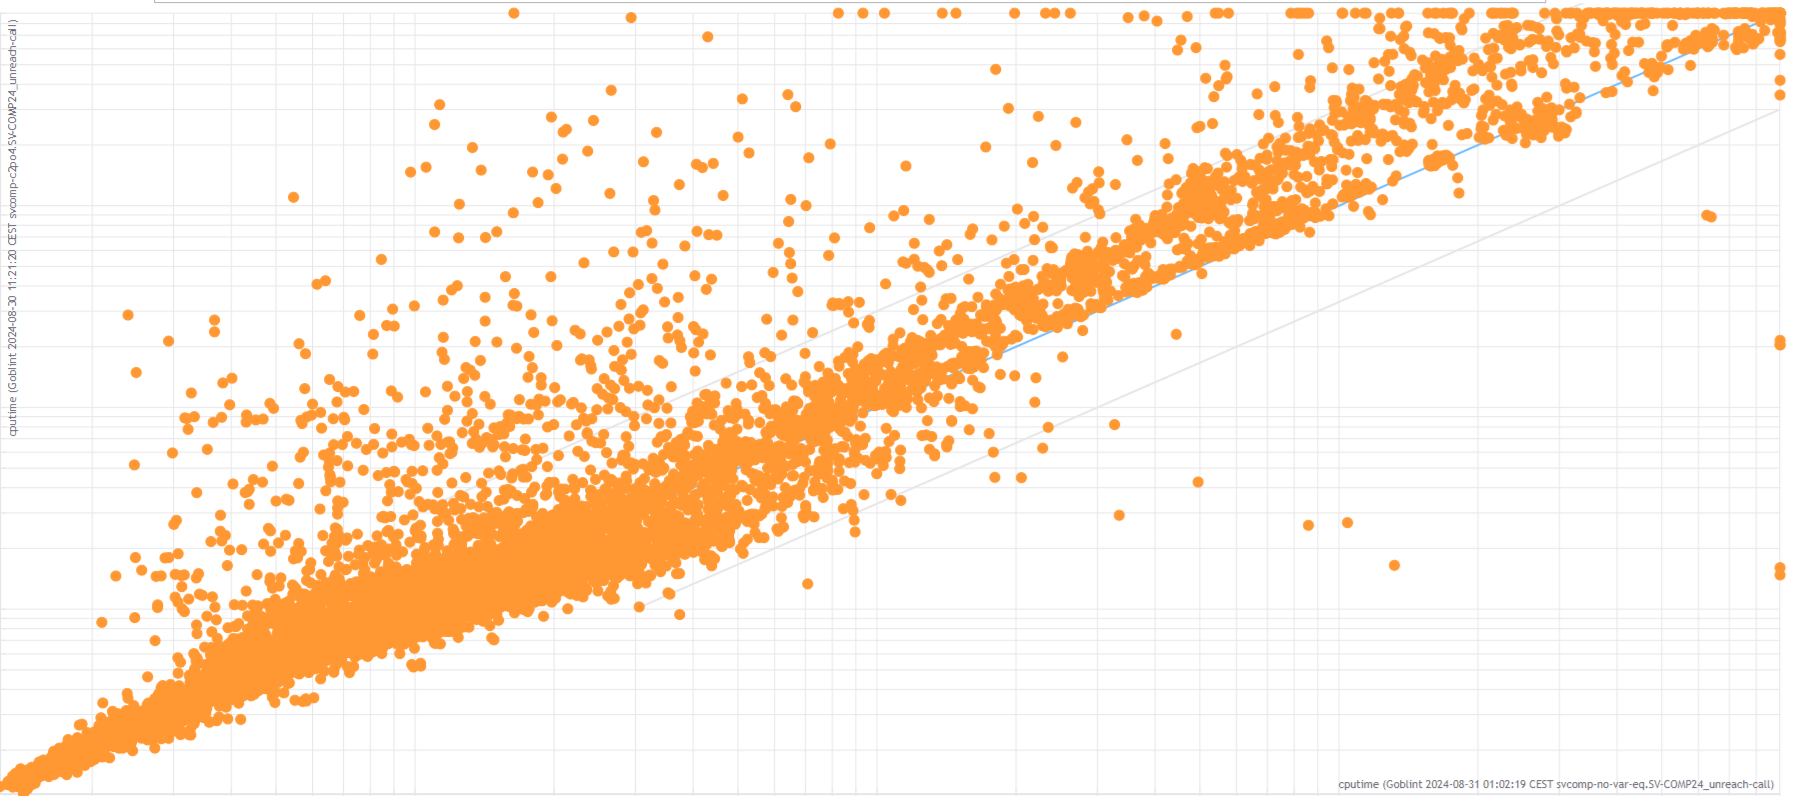
\includegraphics[scale=0.3]{images/base-vs-cpo4-cropped.png}
\end{frame}

\section{Conclusion}
\frame{\tableofcontents[currentsection]}

\begin{frame}{Conclusion}
    \begin{itemize}
        \item \cpo\ can find additional invariants to current \goblint\ analyses
        \item Increase precision by cooperating with non-relational analysis
        \item Could be also the opposite
        \item Find relational properties with relatively small overhead (because of weakly-)
    \end{itemize}
    %was haben wir gelernt, ist sie geeignet, was sind die vorteile
    %man kann auch unsere analyse benutzen um zu wissen, ob sachen bei einem assignment überschrieben werden, so wie wir die non-relational pointer analyse benutzen
\end{frame}

\appendix

\begin{frame}[allowframebreaks]
    \frametitle{References}
    \bibliographystyle{amsalpha}
    \bibliography{main.bib}
\end{frame}


\begin{frame}{Two-dimensional Memory Model}
    \begin{itemize}
        \item In C: pointer arithmetic is not allowed to go outside the current memory object
        \item Address: (blockID, offset)
        \item $bl(a,b) = a$

    \end{itemize}
    \begin{tikzpicture}

        \def\blockheight{0.8}
        \def\startx{0}

        \draw (\startx, 0) rectangle (\startx + 3, -\blockheight);
        \node[anchor=west] at (\startx, -0.5*\blockheight) {int x};
        \draw (\startx, -\blockheight) rectangle (\startx + 5, -2*\blockheight);
        \node[anchor=west] at (\startx, -1.5*\blockheight) {struct a};
        \draw (\startx, -2*\blockheight) rectangle (\startx + 7, -3*\blockheight);
        \node[anchor=west] at (\startx, -2.5*\blockheight) {int a[5]};
        \draw (\startx, -3*\blockheight) rectangle (\startx + 9, -4*\blockheight);
        \node[anchor=west] at (\startx, -3.5*\blockheight) {malloc\#001};

        \draw[->] (\startx,  -4*\blockheight) -- (\startx + 10, -4*\blockheight) node[anchor=north] {Offset};
        \draw[->] (\startx,  -4*\blockheight) -- (\startx, \blockheight) node[anchor=south, rotate=90] {BlockID};

        \node[anchor=east] at (\startx, -1*\blockheight) {3};
        \node[anchor=east] at (\startx, -2*\blockheight) {2};
        \node[anchor=east] at (\startx, -3*\blockheight) {1};
        \node[anchor=east] at (\startx, -4*\blockheight) {0};

        \foreach \x in {0, 2, 4, 6, 8} {
                \draw (\startx + \x, -4*\blockheight) -- (\startx + \x, -4*\blockheight);
                \node[anchor=north] at (\startx + \x, -4*\blockheight) {\x};
            }

    \end{tikzpicture}
\end{frame}

\begin{frame}{Representation of structs and arrays}
    \begin{itemize}
        \item $a[1]\equiv *(a+1)$
        \item $a[i][j] \equiv (a + (i \cdot m + j) \cdot 32) \quad \text{for \texttt{int a[n][m]}}$
        \item struct $s$: $s.f \equiv *(\&s + 32)$
    \end{itemize}
\end{frame}

\begin{frame}{Overlapping values}

    {
        \centering

        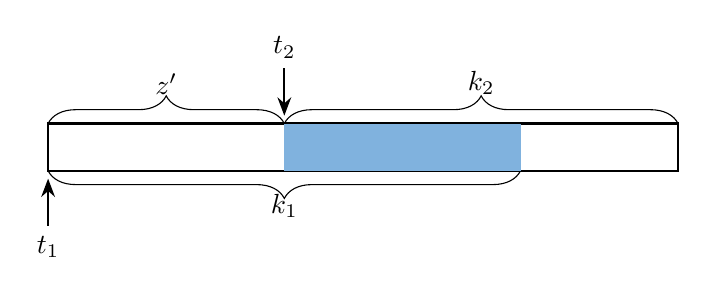
\begin{tikzpicture}[
                memory/.style={draw, thick, minimum height=0.6cm},
                pointer/.style={-Stealth, thick},
                bracket/.style={decorate,decoration={brace, amplitude=10pt, mirror}},
                bracketabove/.style={decorate,decoration={brace, amplitude=10pt}}
            ]

            \draw[memory] (0,0) rectangle (8,0.6);

            \draw[pointer] (3, 1.3) node[above] {$t_2$} -- (3, 0.7);
            \draw[pointer] (0, -0.7) node[below] {$t_1$} -- (0, -0.1);

            \draw[bracketabove] (3, 0.6) -- node[above=7pt] {$k_2$} (8, 0.6);
            \draw[bracketabove] (0, 0.6) -- node[above=7pt] {$z'$} (3, 0.6);
            \draw[bracket] (0, 0) -- node[below=5pt] {$k_1$} (6, 0);

            \draw[dashed] (3, 0) -- (3, 0.6);
            \draw[dashed] (6, 0) -- (6, 0.6);

            \fill[TUMBlue!50] (3,0) rectangle (6,0.6); % overlap

        \end{tikzpicture}
    }
    \begin{itemize}
        \item $t_2 \equiv_{k} z' + t_1$.
        \item There is an overlap if $z' < k_1$.
    \end{itemize}

\end{frame}



\begin{frame}{Equality}
    \todo[inline]{partial order}
    \begin{Definition}
        Eine Definition
    \end{Definition}
\end{frame}



\begin{frame}{Equality}
    How to add equalities:
\end{frame}

\begin{frame}{Interprocedural}
    enter:
    \begin{itemize}
        \item Remove local variables of caller.
        \item Add shadow variable $p'$ for each parameter $p$ and the equality $p = p'$.
    \end{itemize}
    combine:
    \begin{itemize}
        \item Remove tainted variables from caller state.
        \item Meet caller and callee state.
        \item Add equality $p' = e$ for each parameter $p$ called with the expression $e$.
        \item Assign return value to variable if necessary.
        \item Remove local variables of callee and shadow variables.
    \end{itemize}
\end{frame}


\end{document}
